\chapter{Лабораторная работа}

\section*{Цель работы}

Лабораторная работа №3 выполняется на основе лабораторной работы № 2. Ее цель заключается в отработке навыков использования программы Microsoft Project для оптимизации временных и финансовых показателей проекта.

\section*{Содержание проекта}

Команда разработчиков из 16 человек занимается созданием карты города на основе собственного модуля отображения. Проект должен быть завершен в течение 6 месяцев. Бюджет проекта: 50 000 рублей.

\section*{Задание 1: Выравнивание загрузки ресурсов в проекте}

Параметры выравнивания:

\begin{figure}[H]
	\begin{center}
		
\includegraphics[width=0.7\textwidth]{imgs/task_1_0.png}
	\end{center}
\end{figure}

После выравнивания работники больше не перегружены:

\begin{figure}[H]
	\begin{center}
		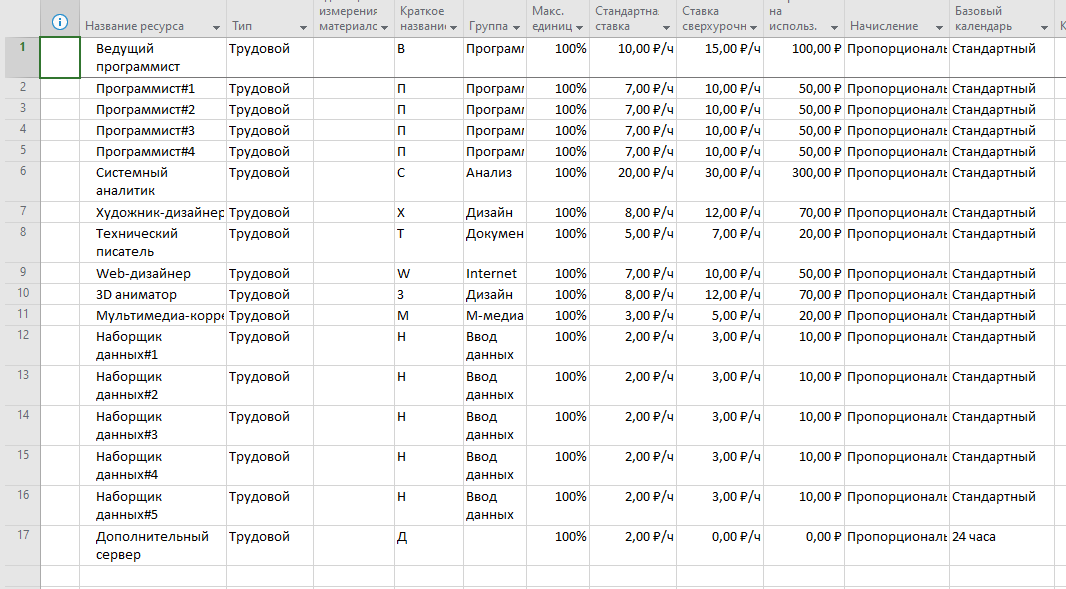
\includegraphics[width=\textwidth]{imgs/task_1_1.png}
	\end{center}
\end{figure}

До выравнивания:

\begin{figure}[H]
	\begin{center}
		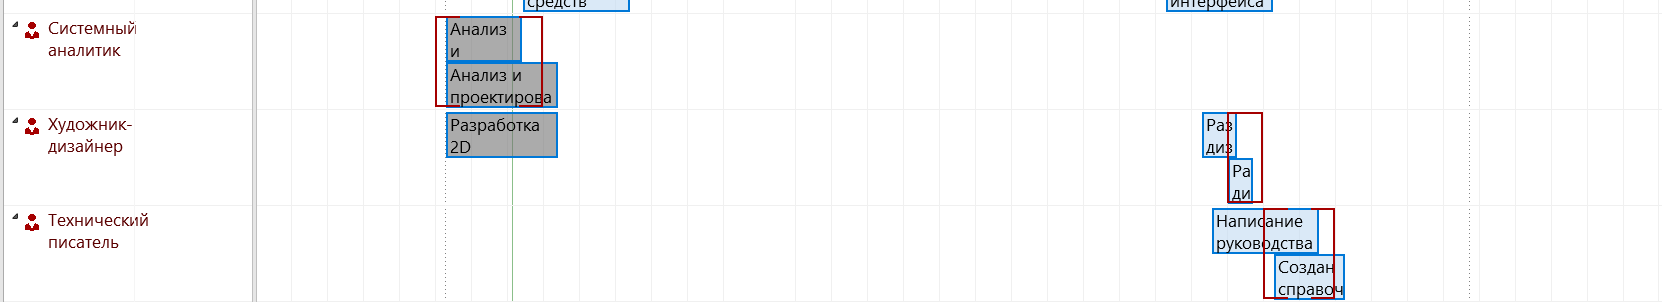
\includegraphics[width=\textwidth]{imgs/task_1_2.png}
	\end{center}
\end{figure}

После выравнивания:

\begin{figure}[H]
	\begin{center}
		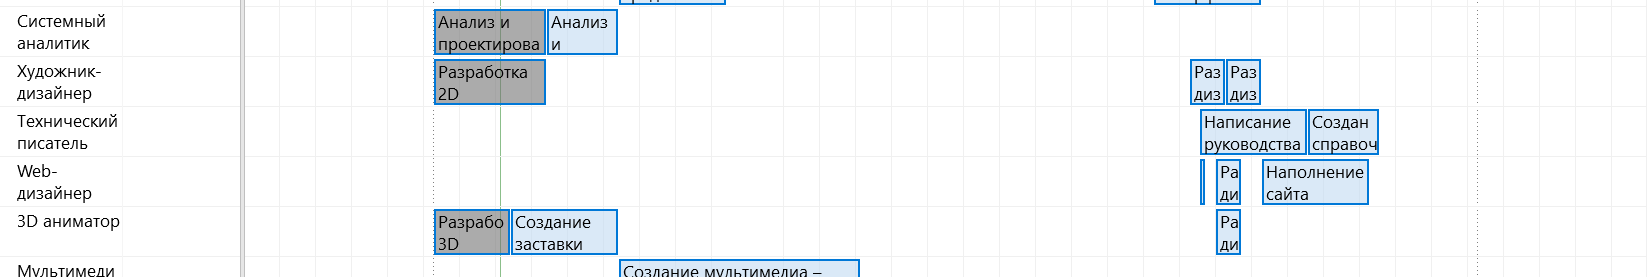
\includegraphics[width=\textwidth]{imgs/task_1_3.png}
	\end{center}
\end{figure}

\section*{Задание 2: Учет периодических задач в плане проекта}

Добавим еженедельную задачу <<Совещание>> длительностью 1 час по средам

\begin{figure}[H]
	\begin{center}
		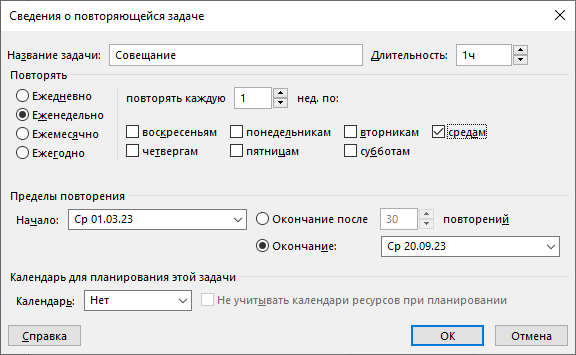
\includegraphics[width=0.8\textwidth]{imgs/task_2_0.png}
	\end{center}
\end{figure}

Результат:

\begin{figure}[H]
	\begin{center}
		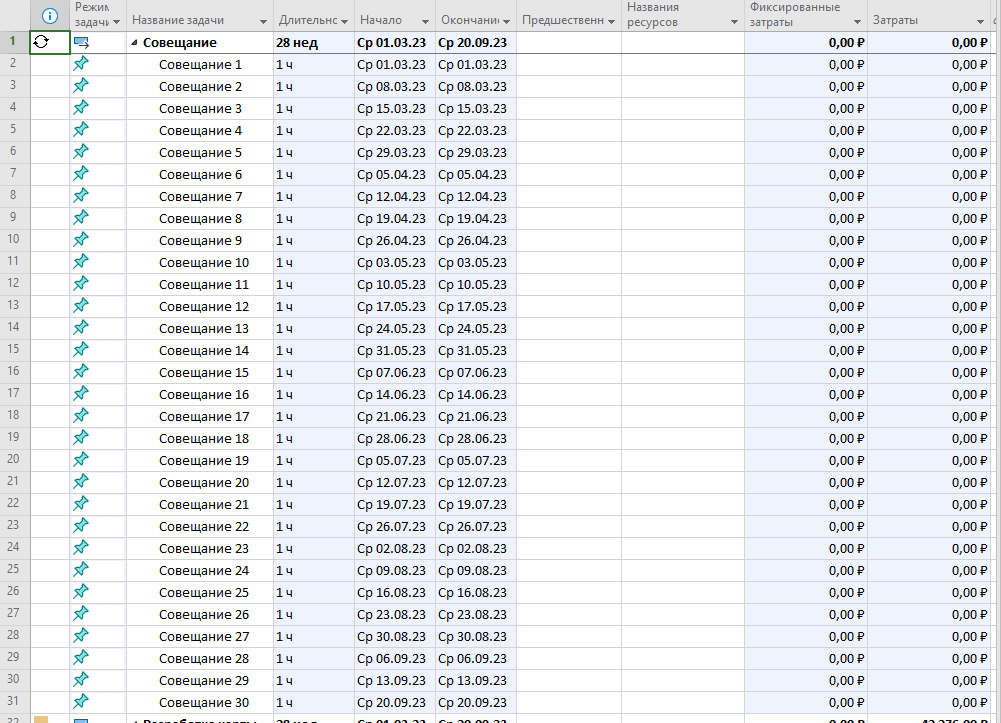
\includegraphics[width=\textwidth]{imgs/task_2_1.png}
	\end{center}
\end{figure}

Добавим участников совещания:

\begin{figure}[H]
	\begin{center}
		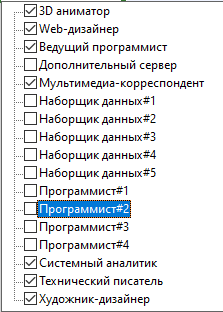
\includegraphics[width=0.3\textwidth]{imgs/task_2_2.png}
	\end{center}
\end{figure}

В результате этого проект вышел за бюджет в 50 000 рублей, увеличились сроки.

\begin{figure}[H]
	\begin{center}
		
\includegraphics[width=\textwidth]{imgs/task_2_3.png}
	\end{center}
\end{figure}

\begin{figure}[H]
	\begin{center}
		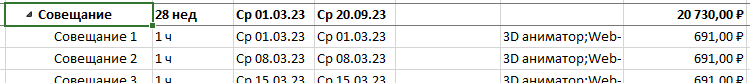
\includegraphics[width=\textwidth]{imgs/task_2_4.png}
	\end{center}
\end{figure}

Превышение бюджета связано с тем, что участники совещания тратят рабочий час на совещания, который оплачивается также, вследствии чего увеличиваются сроки выполнения проекта, а значит растет и бюджет.

У всех участников совещаний была добавлена таблица затрат B.

\begin{figure}[H]
	\begin{center}
		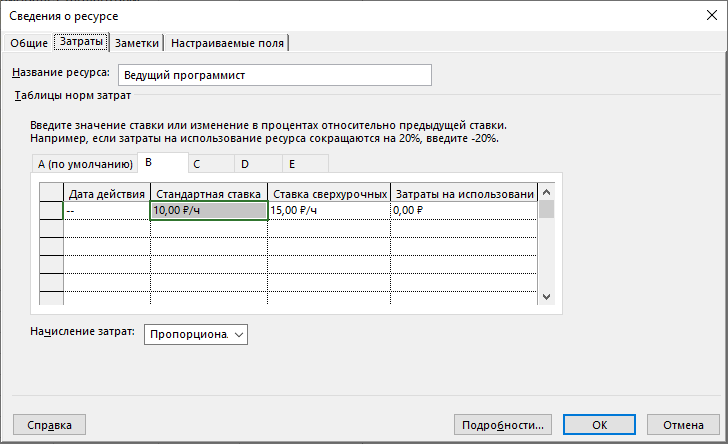
\includegraphics[width=0.7\textwidth]{imgs/task_2_5.png}
	\end{center}
\end{figure}

Установим всем совещающимся таблицу норм затрат B.

\begin{figure}[H]
	\begin{center}
		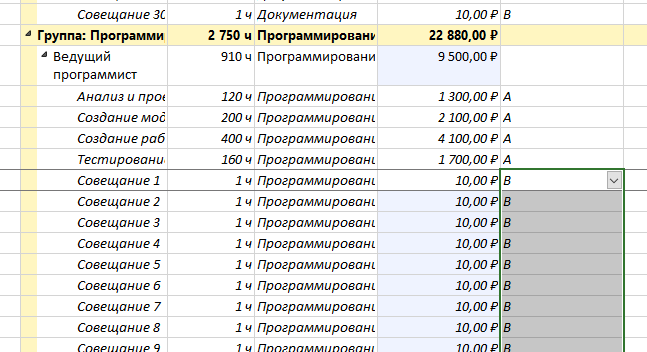
\includegraphics[width=0.8\textwidth]{imgs/task_2_6.png}
	\end{center}
\end{figure}

Заметим, что затраты на совещания поменялись.

\begin{figure}[H]
	\begin{center}
		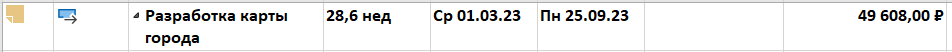
\includegraphics[width=\textwidth]{imgs/task_2_7.png}
	\end{center}
\end{figure}

\begin{figure}[H]
	\begin{center}
		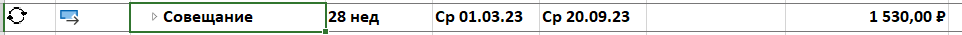
\includegraphics[width=\textwidth]{imgs/task_2_8.png}
	\end{center}
\end{figure}

\section*{Задание 3: Оптимизация критического пути}

Отобразим критические задачи:

\begin{figure}[H]
	\begin{center}
		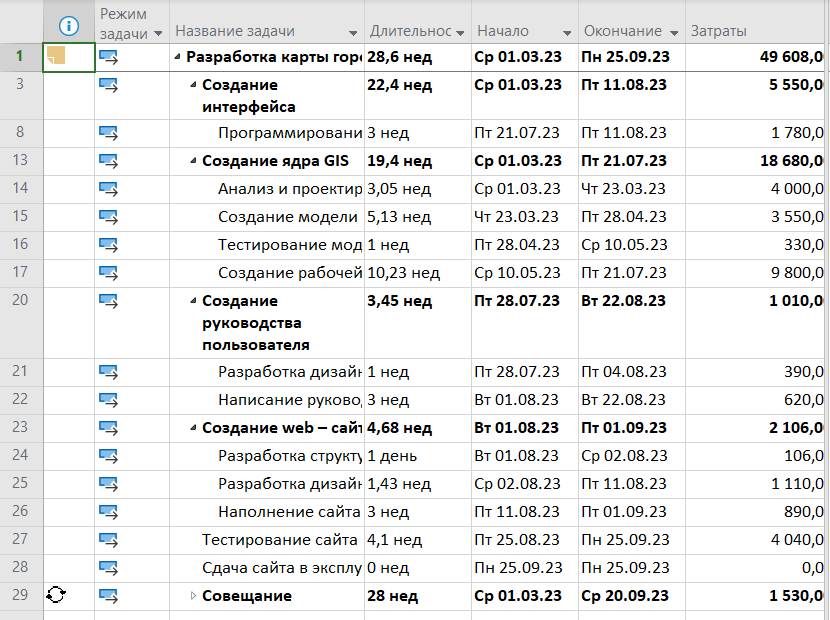
\includegraphics[width=\textwidth]{imgs/task_3_0.png}
	\end{center}
\end{figure}

\begin{figure}[H]
	\begin{center}
		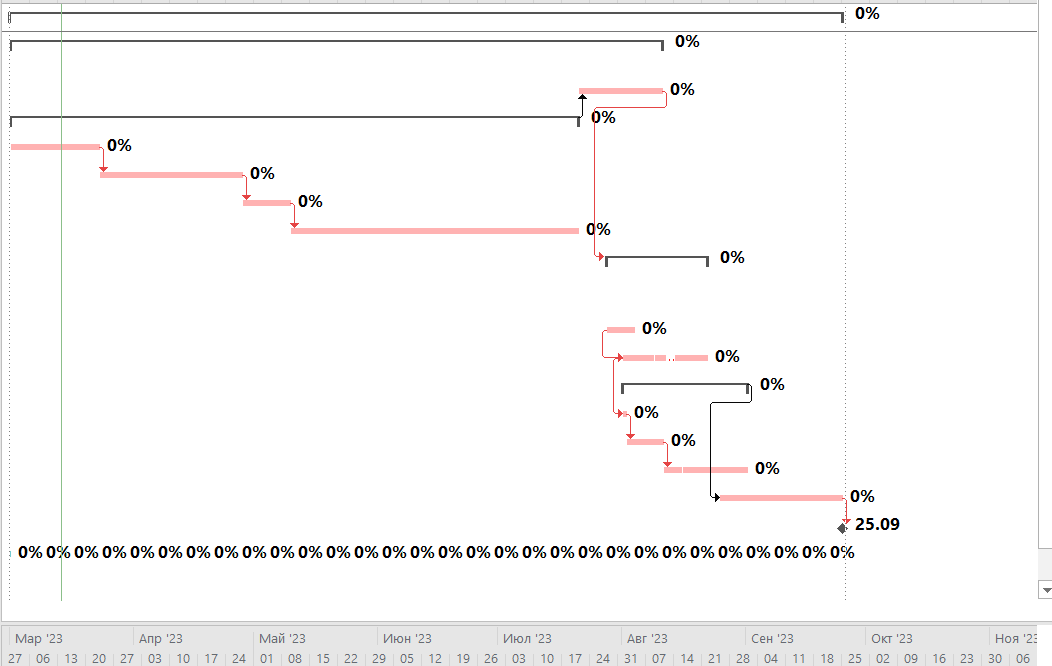
\includegraphics[width=\textwidth]{imgs/task_3_1.png}
	\end{center}
\end{figure}

Добавим задачам <<Создание модели ядра>> и <<Создание рабочей версии ядра>> всех программистов. Таким образом мы уменьшили длительность задач, тем самым сократили длительность проекта до 24.61 недель.

\begin{figure}[H]
	\begin{center}
		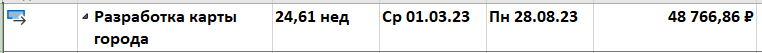
\includegraphics[width=\textwidth]{imgs/task_3_2.png}
	\end{center}
\end{figure}

Сравним <<Трудозатраты -- затраты>> до и после оптимизации.

До оптимизации:

\begin{figure}[H]
	\begin{center}
		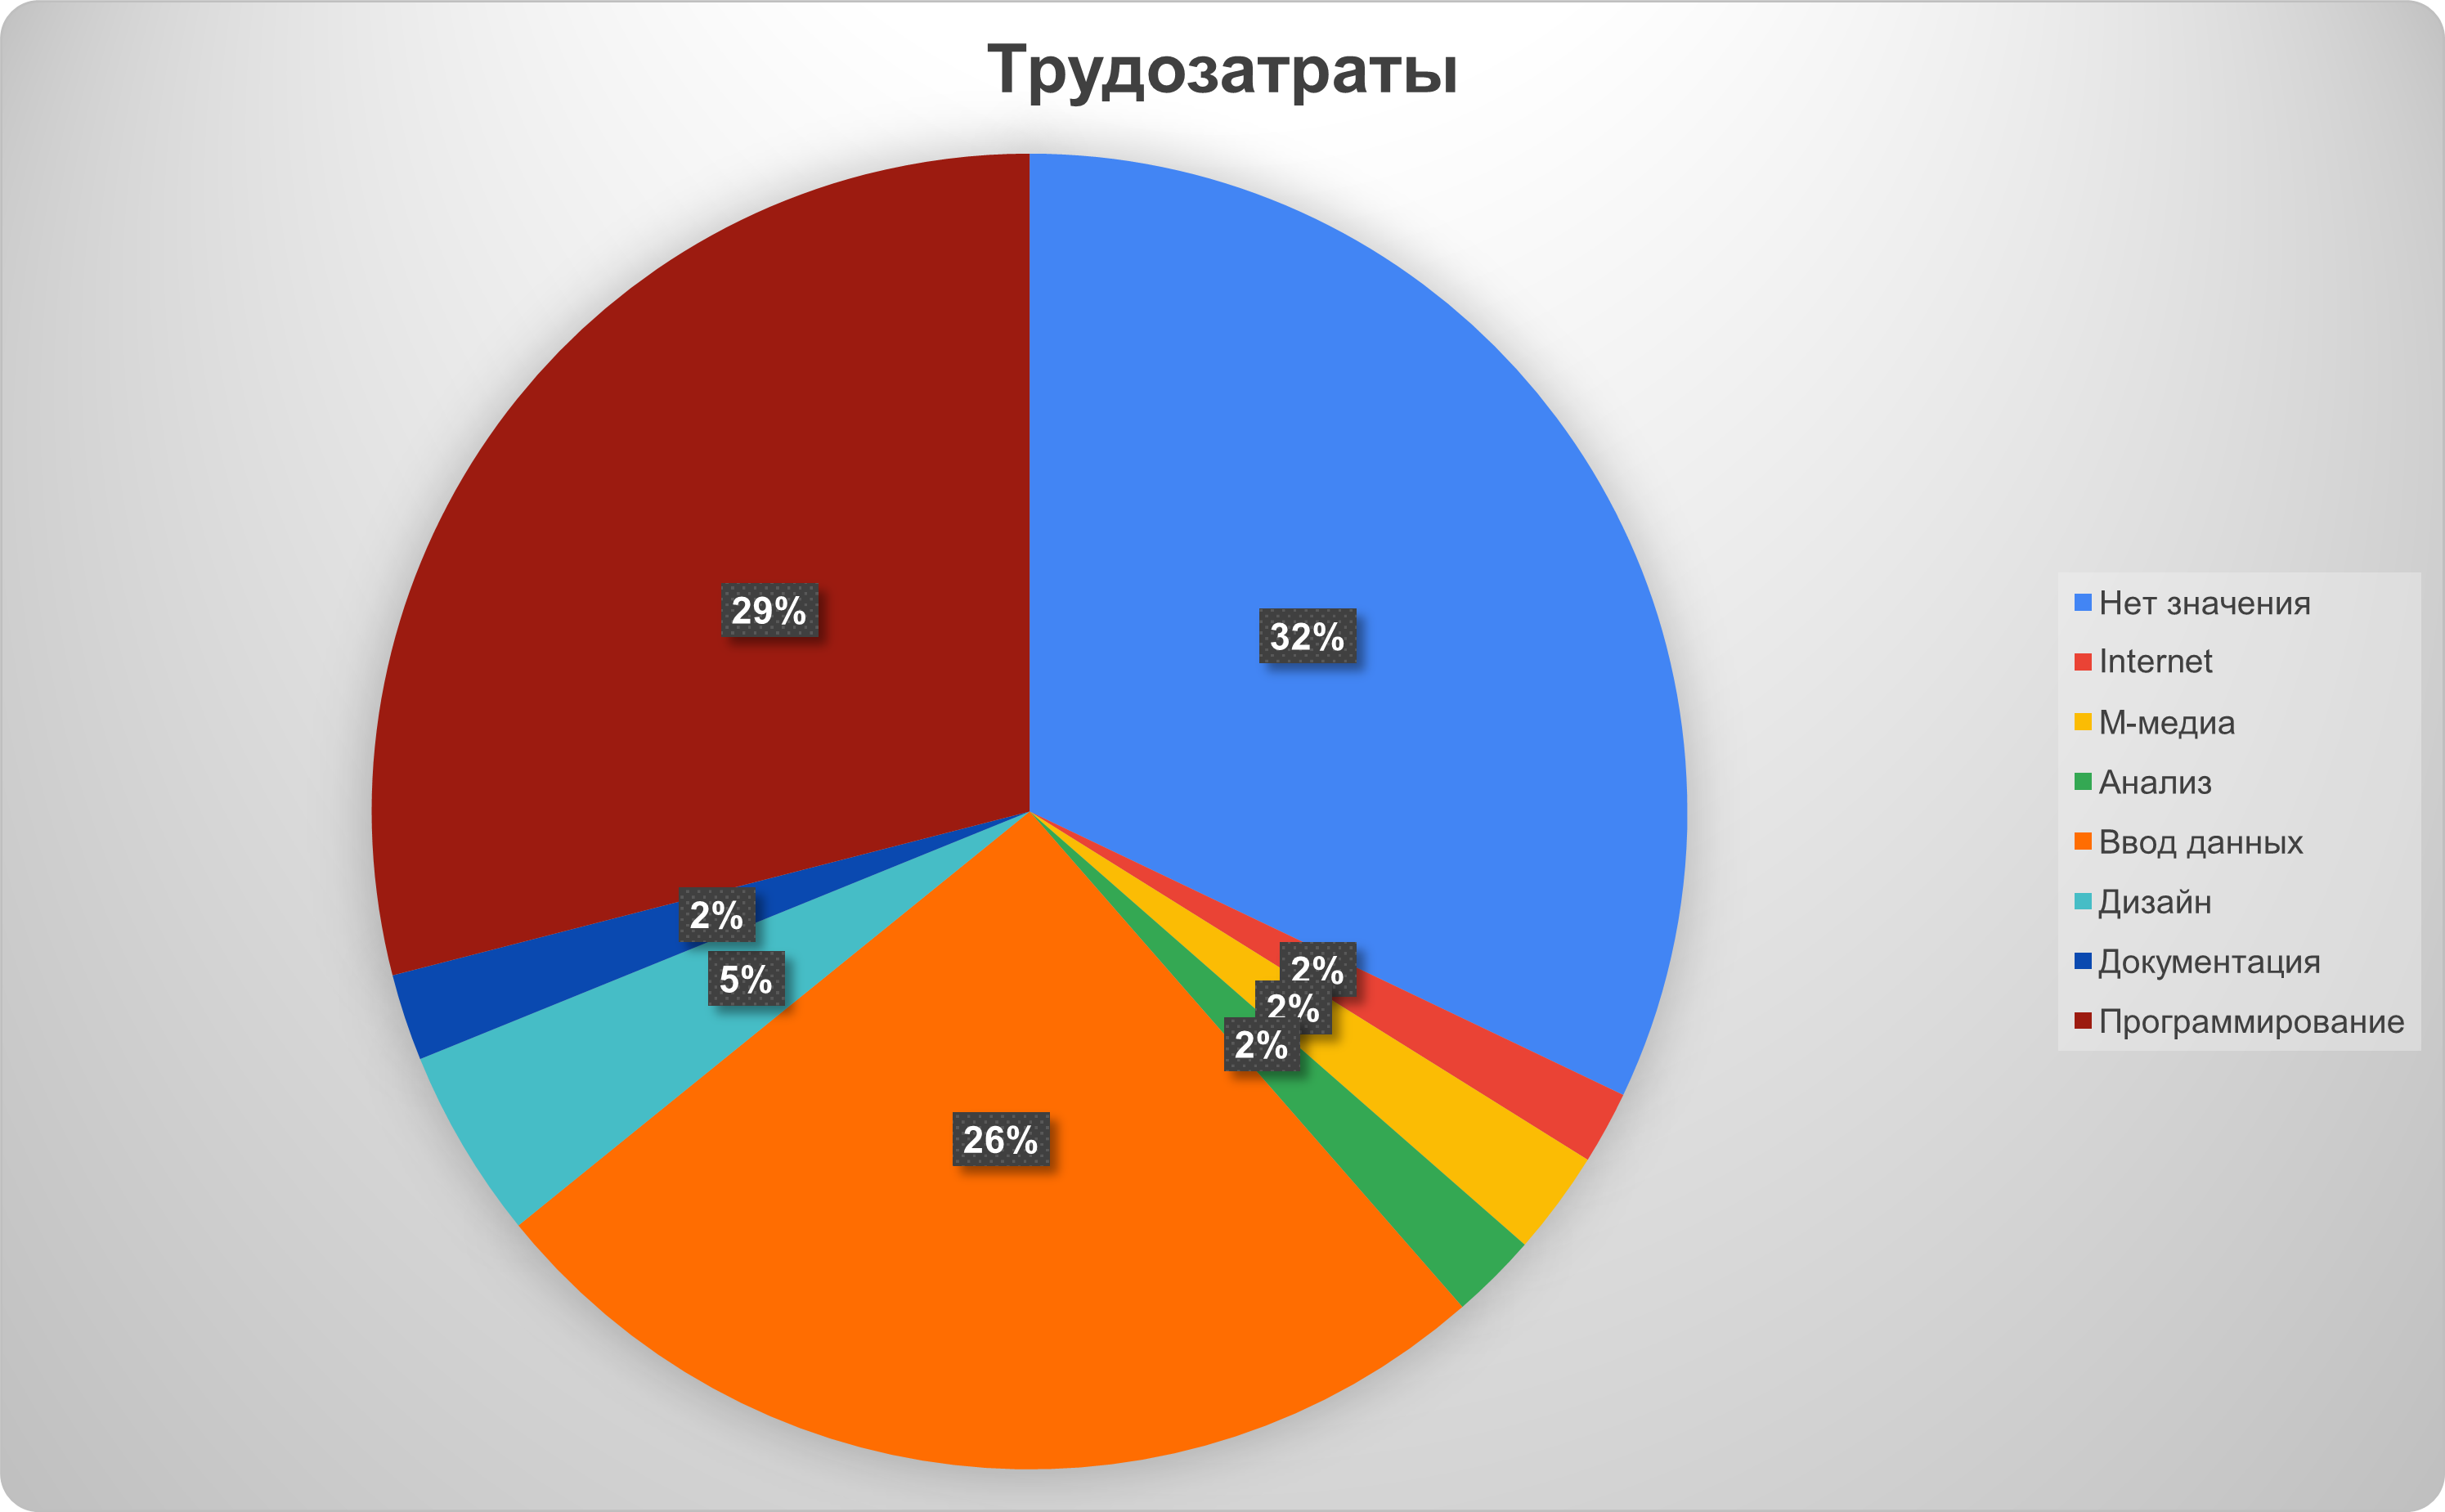
\includegraphics[width=\textwidth]{imgs/task_3_4.png}
	\end{center}
\end{figure}

\begin{figure}[H]
	\begin{center}
		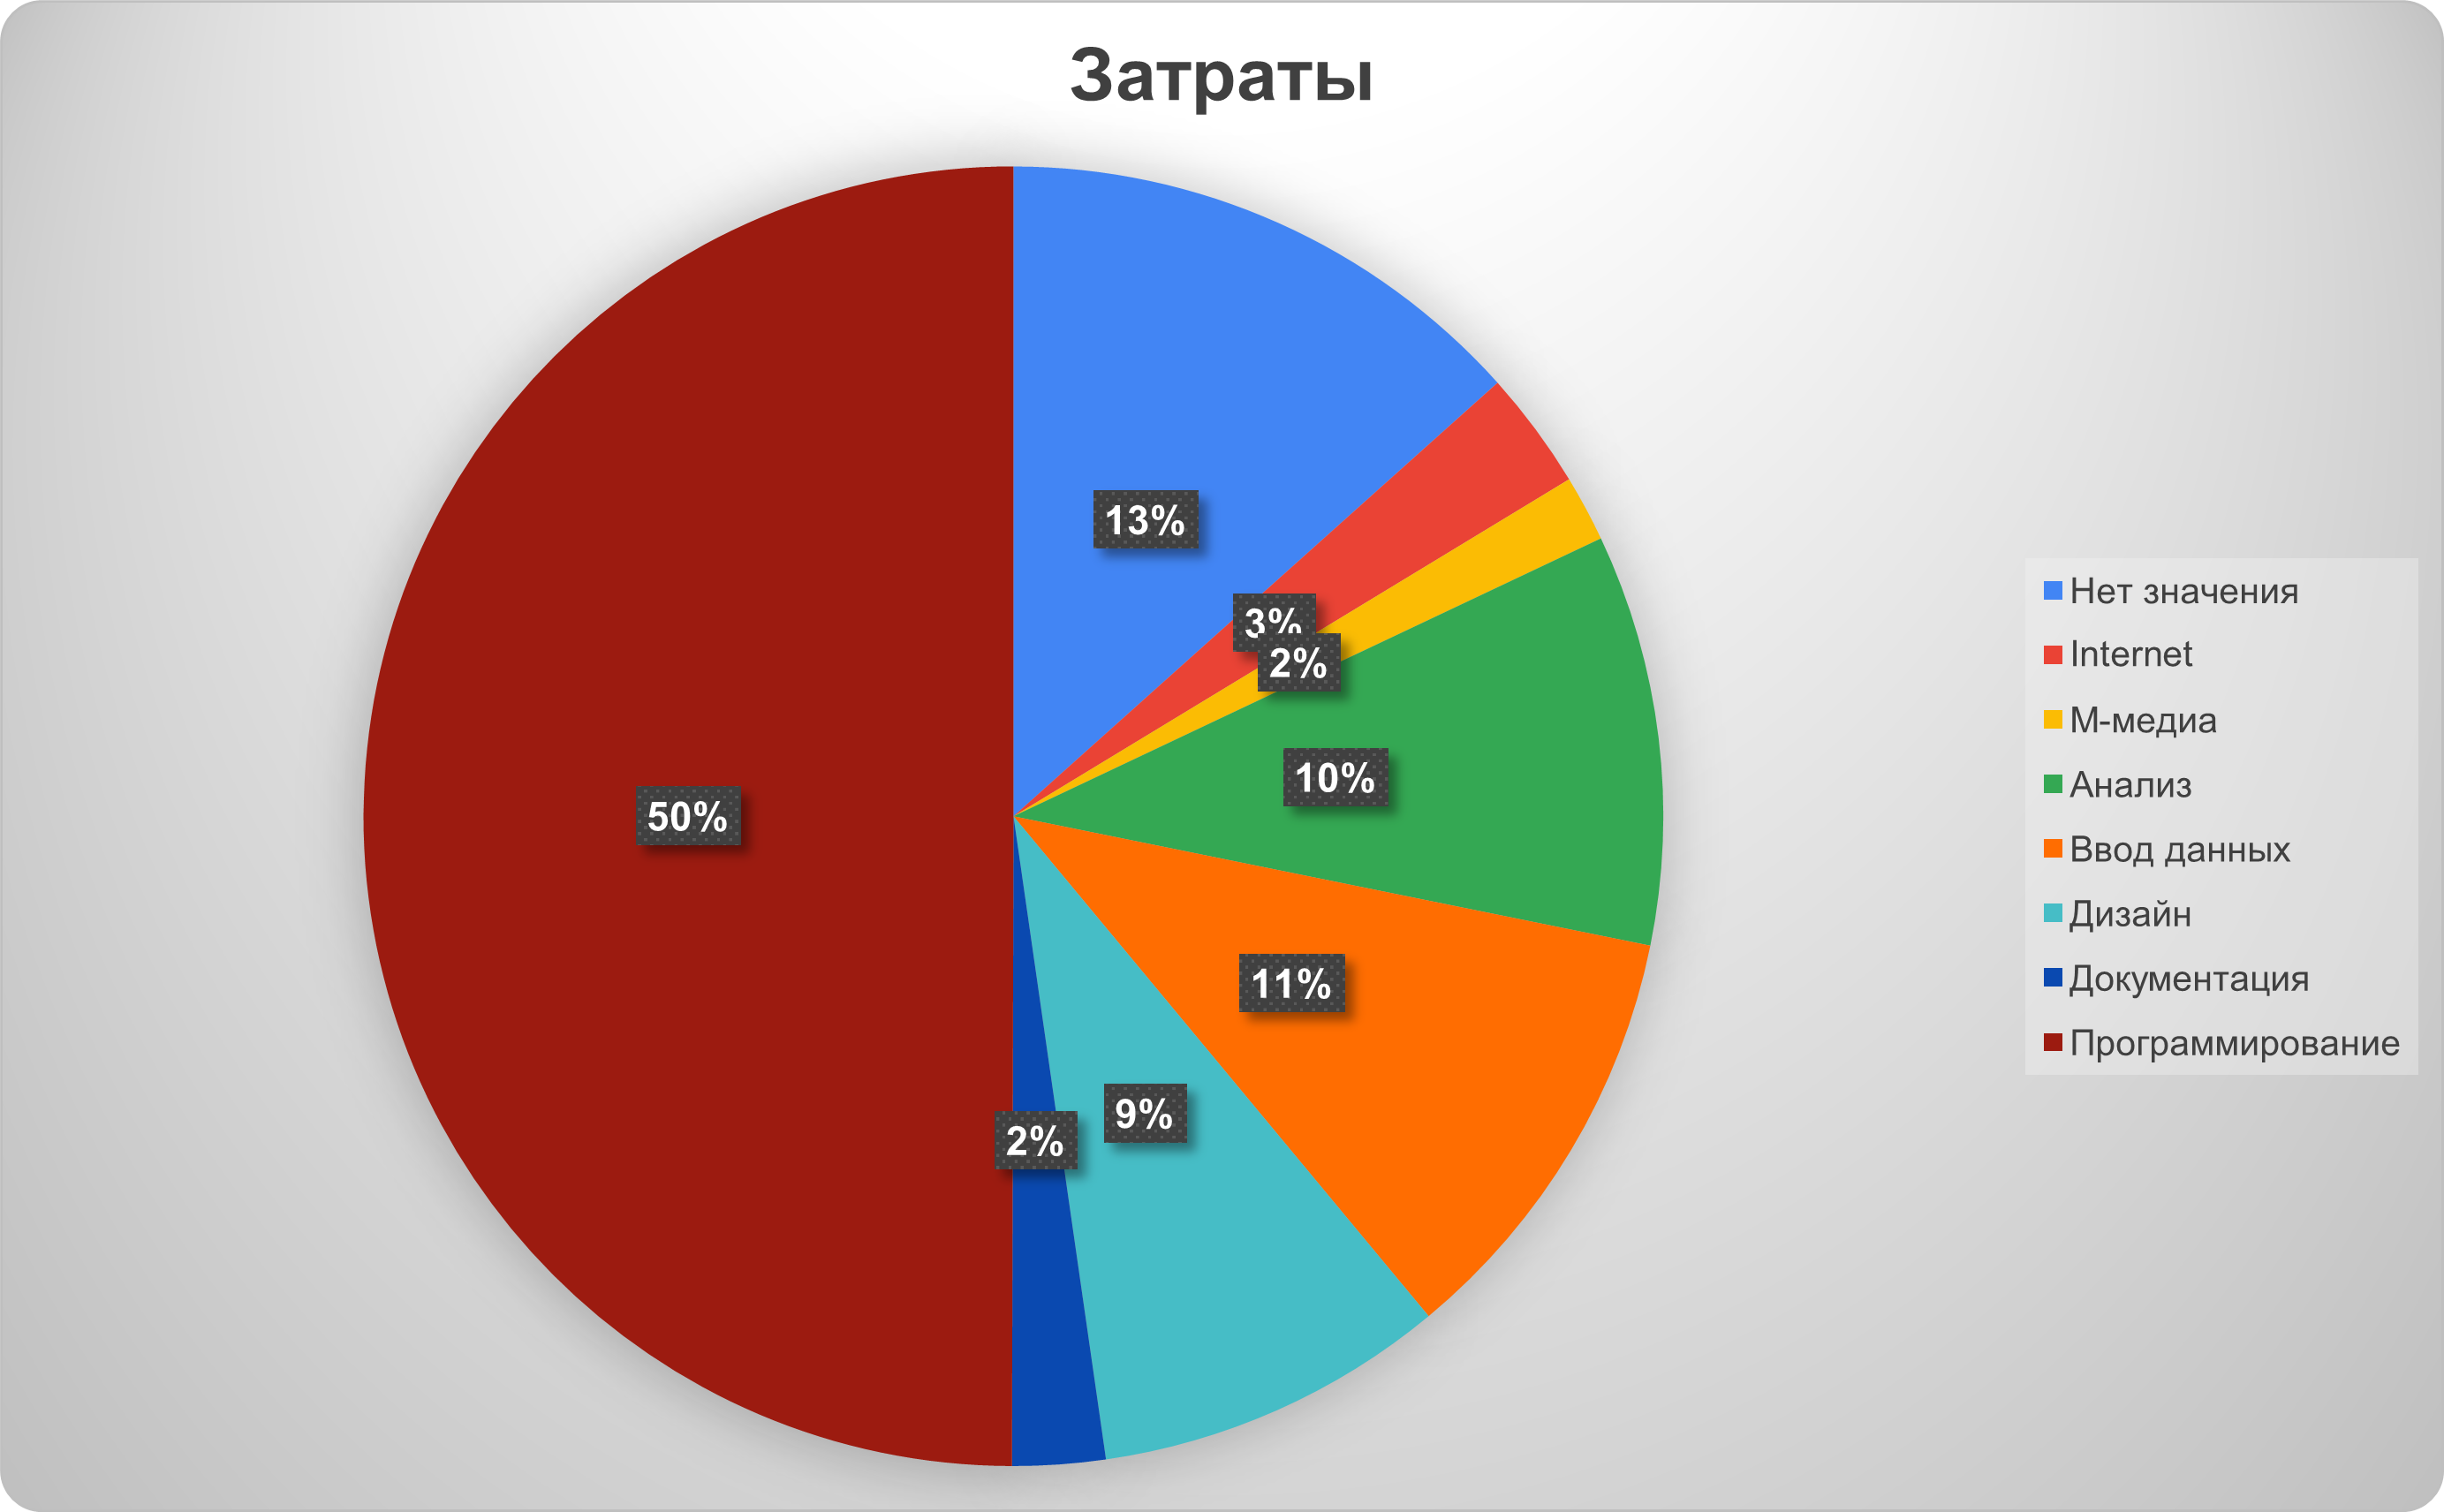
\includegraphics[width=\textwidth]{imgs/task_3_5.png}
	\end{center}
\end{figure}

После оптимизации:

\begin{figure}[H]
	\begin{center}
		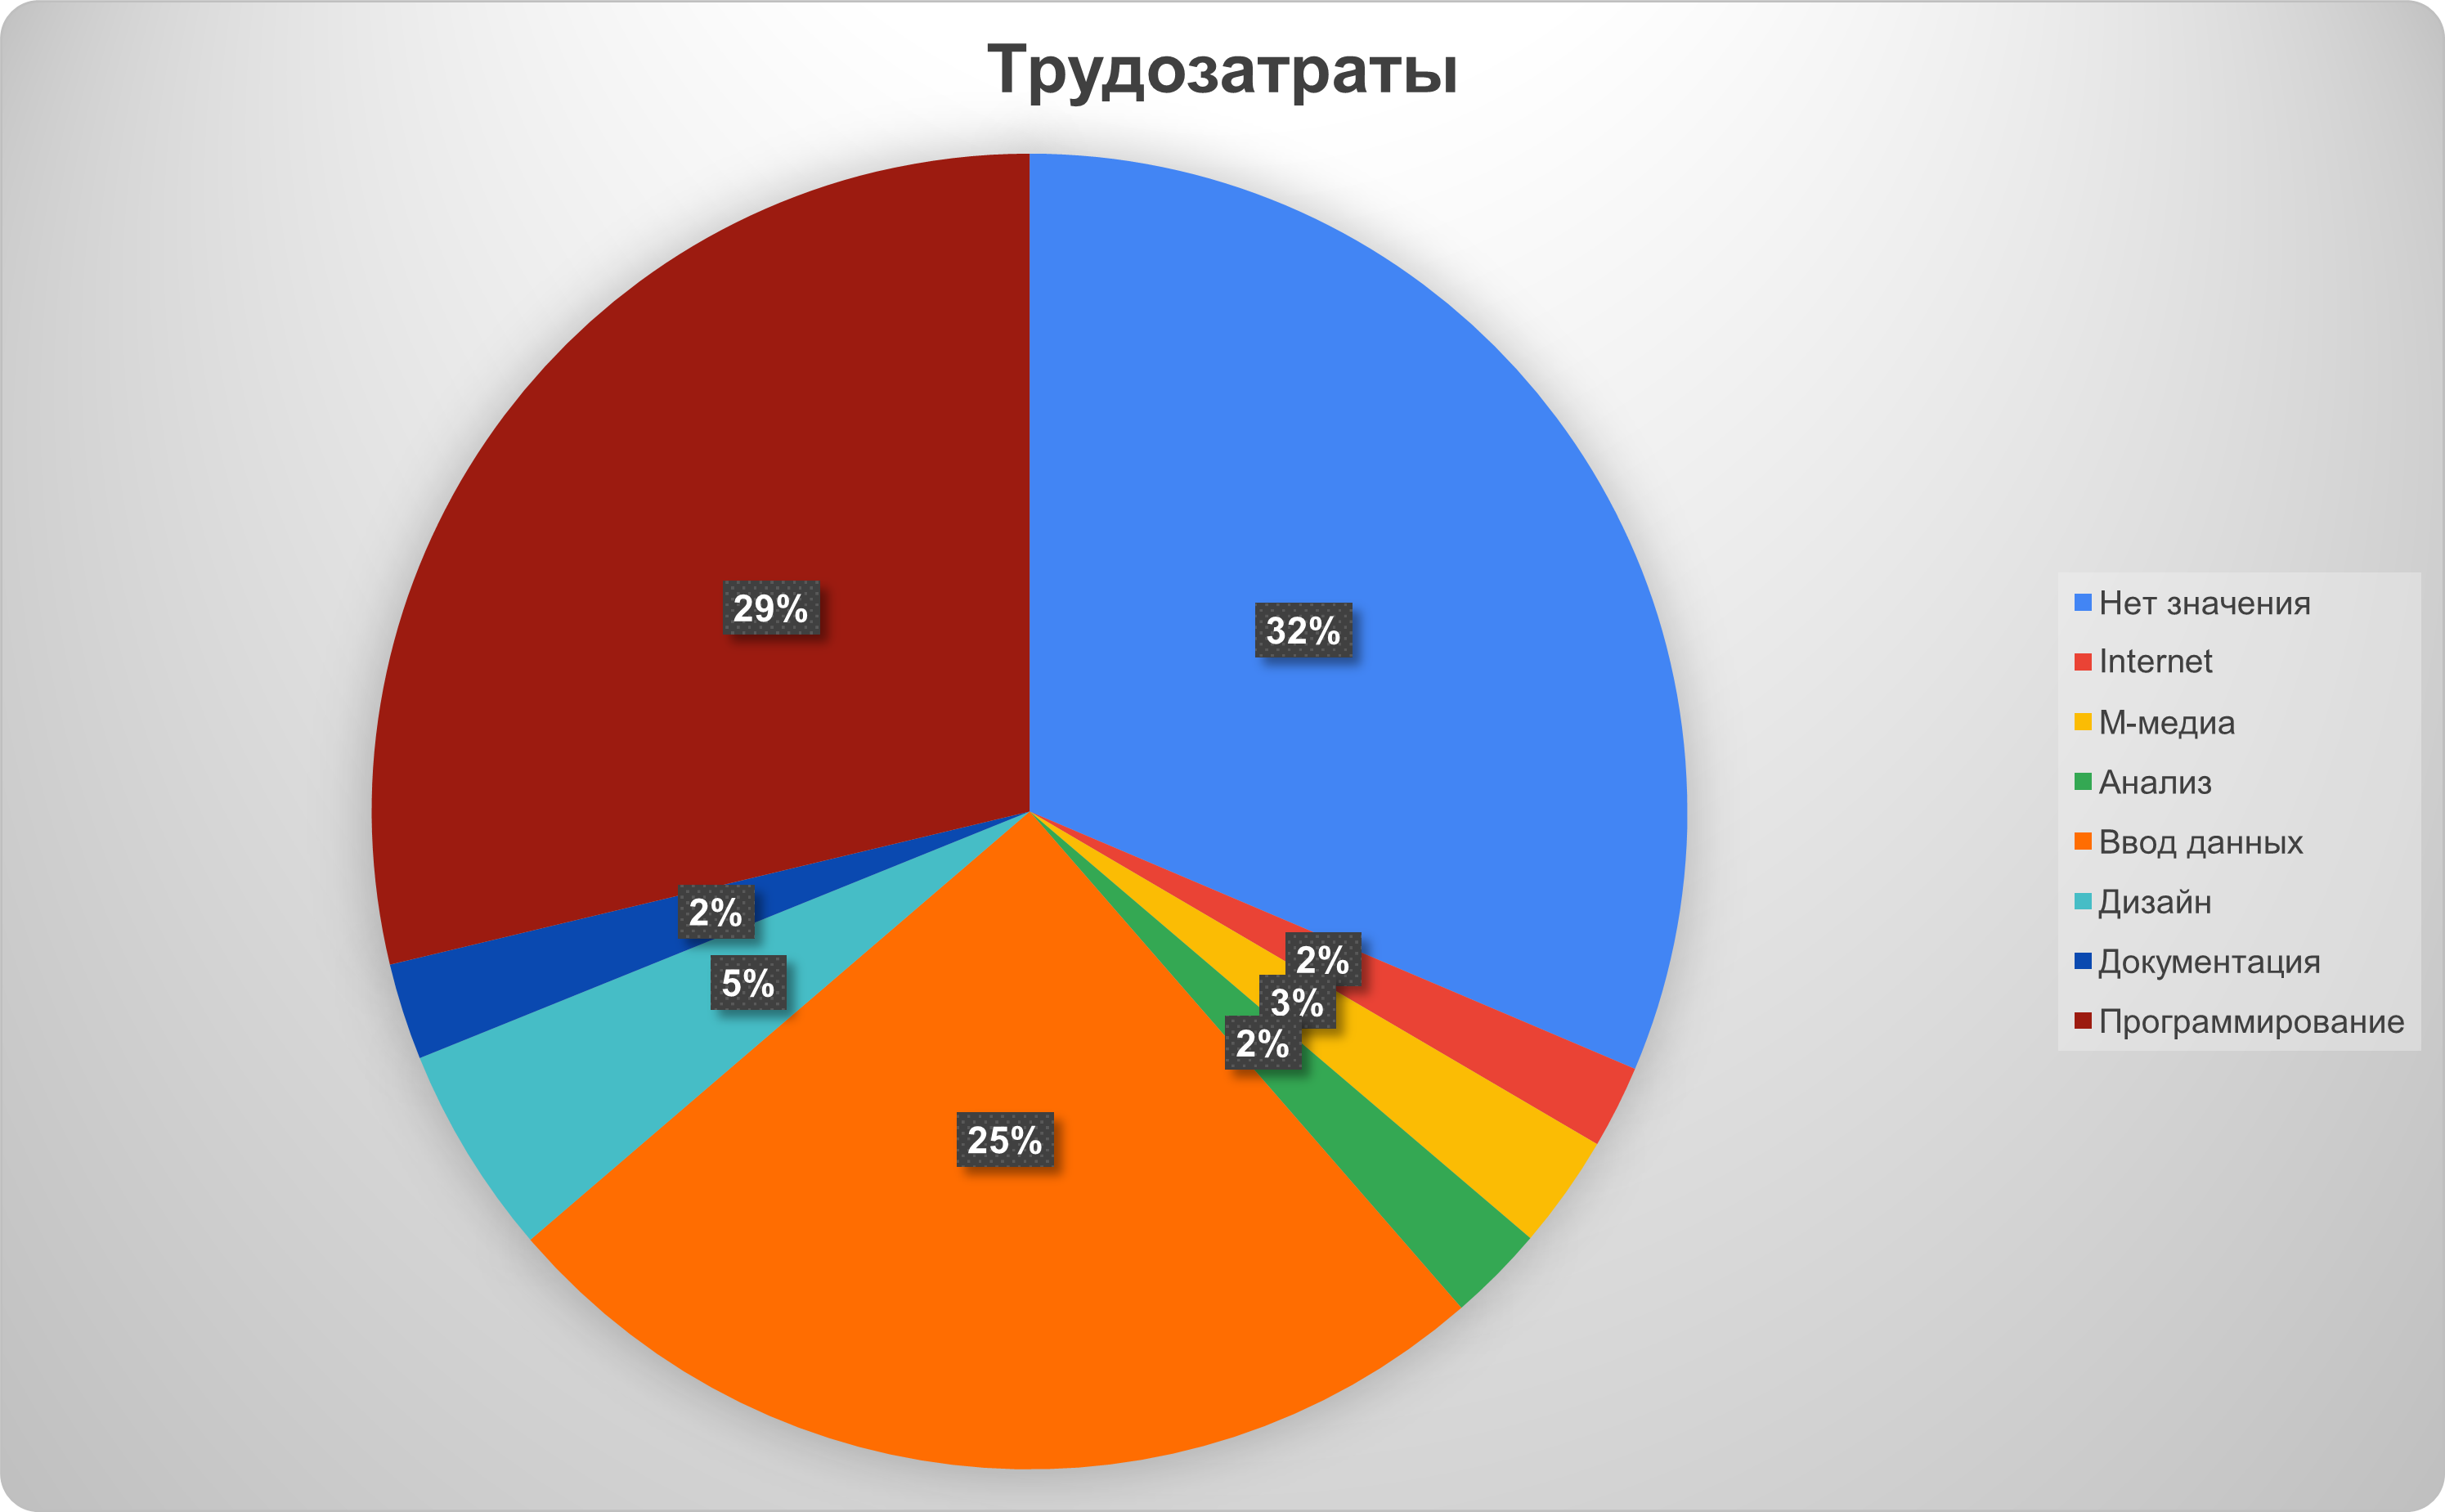
\includegraphics[width=\textwidth]{imgs/task_3_6.png}
	\end{center}
\end{figure}

\begin{figure}[H]
	\begin{center}
		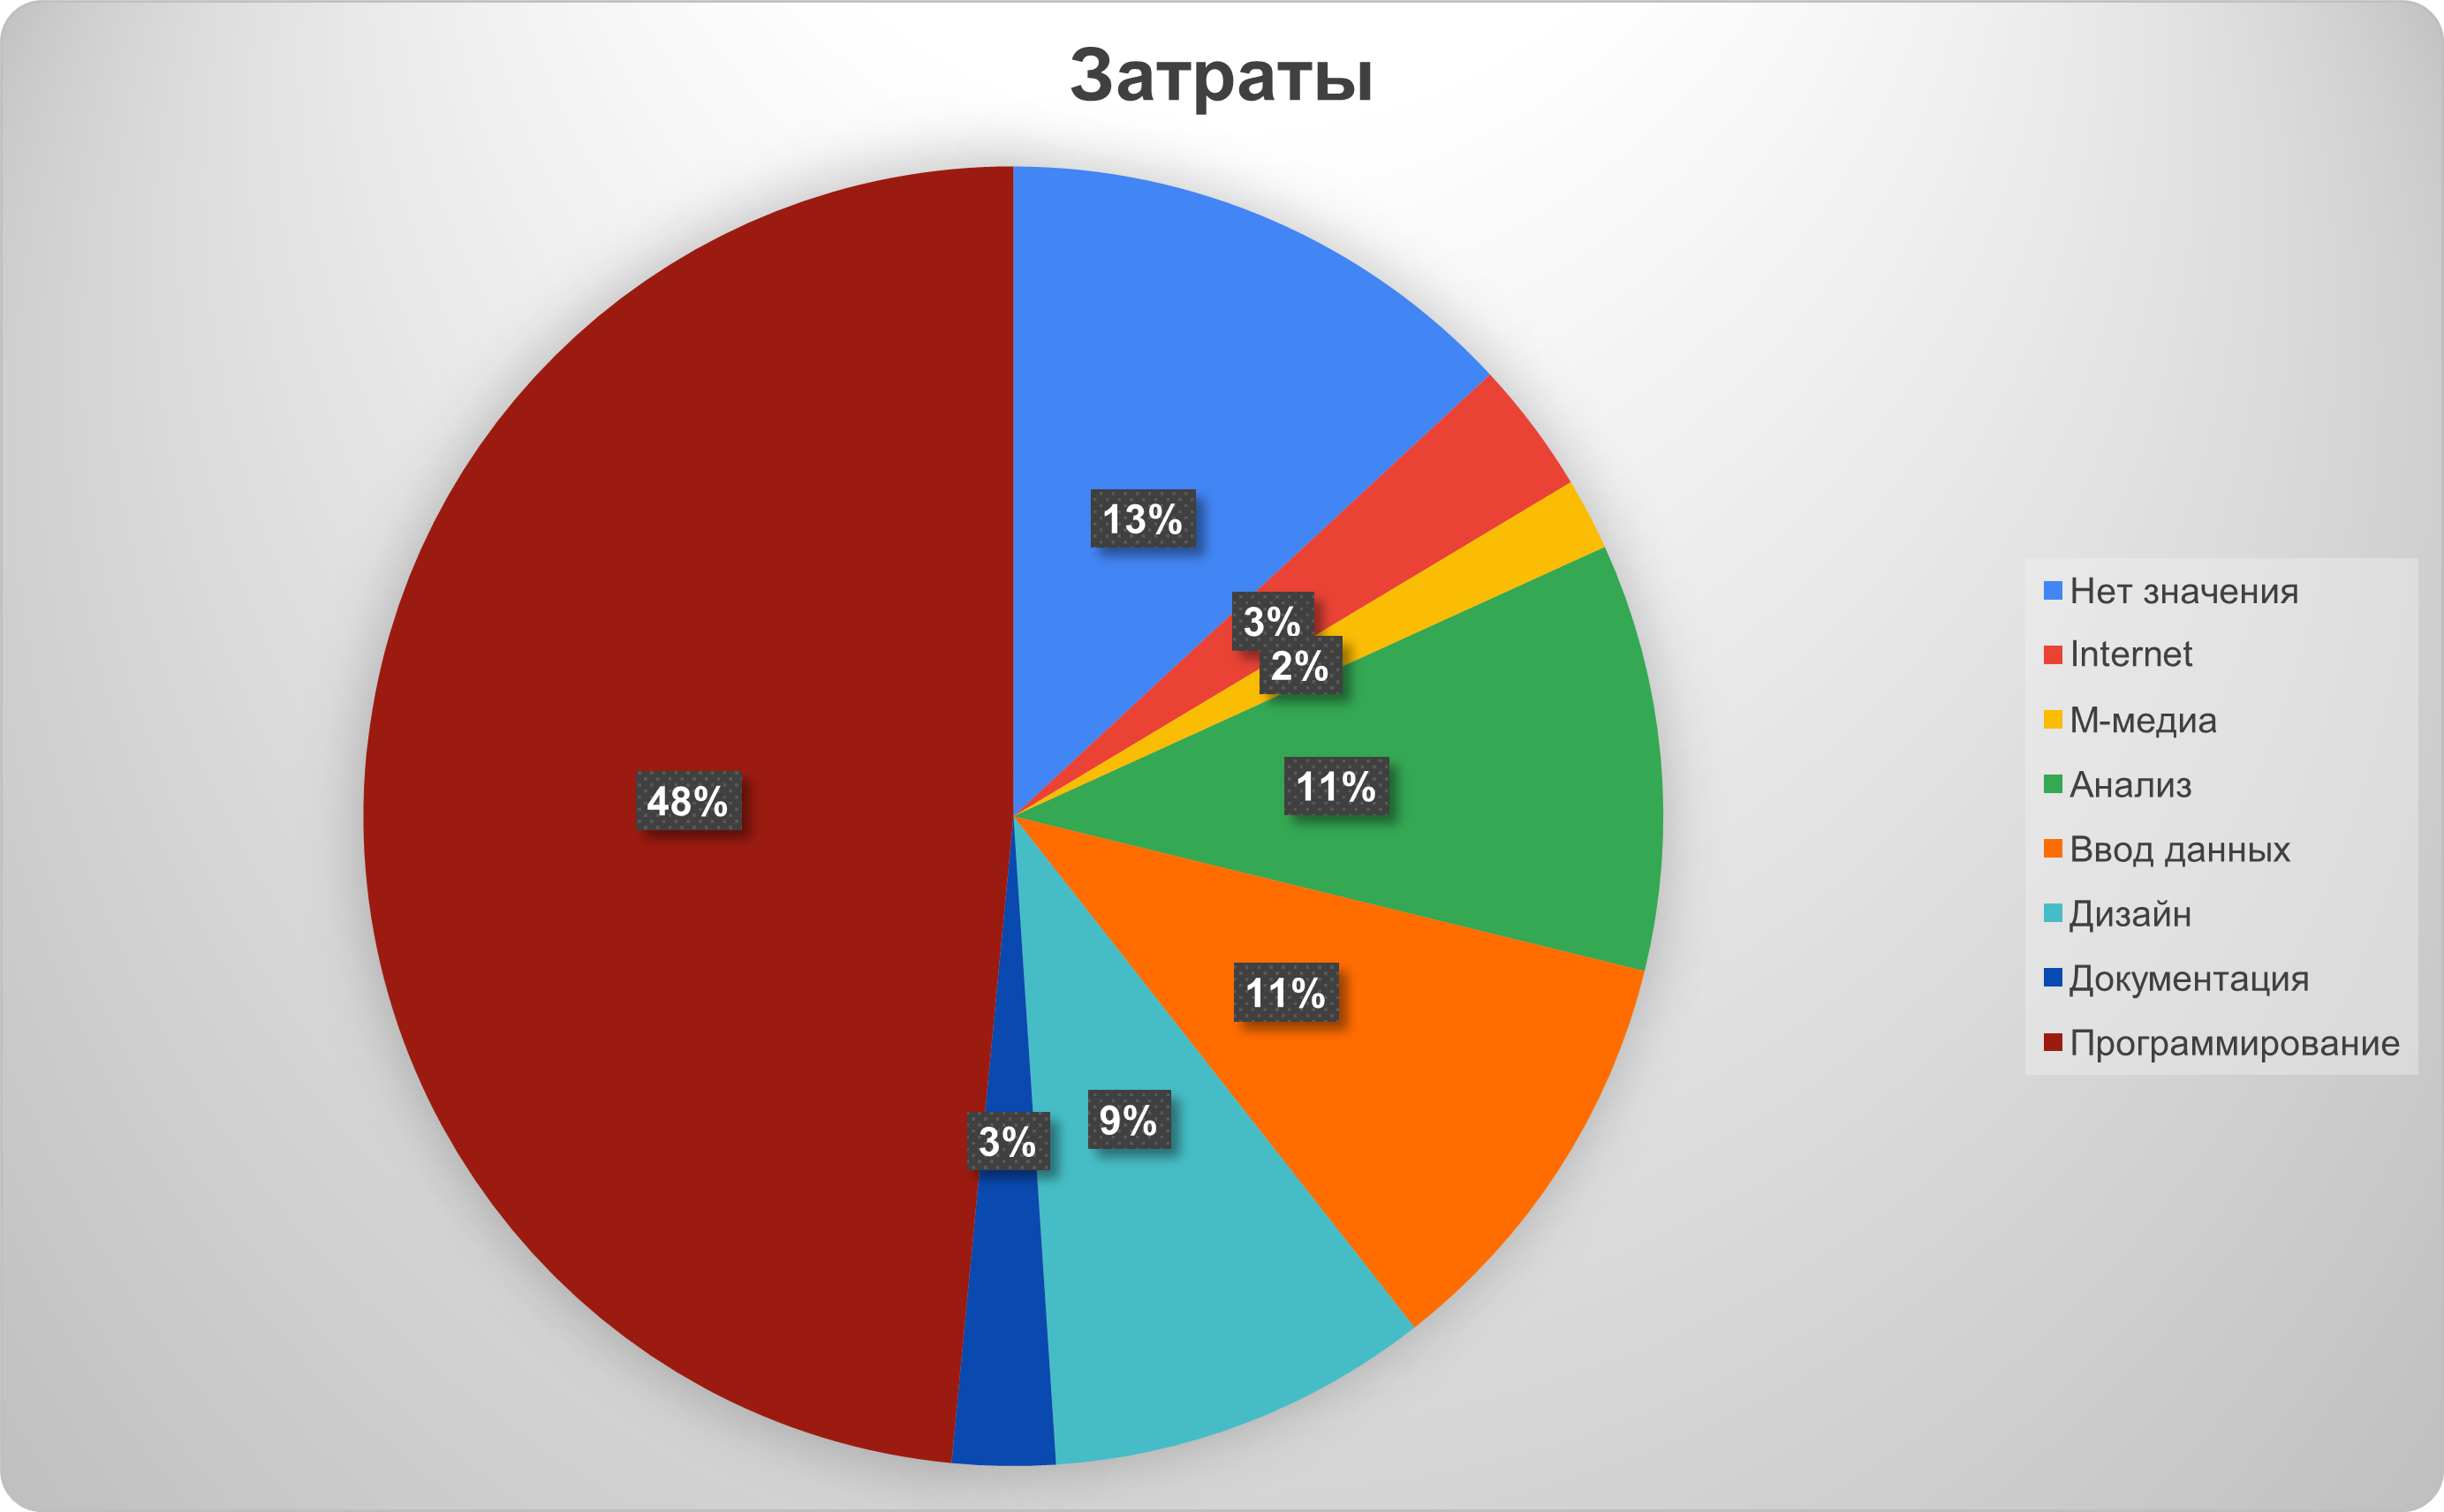
\includegraphics[width=\textwidth]{imgs/task_3_7.png}
	\end{center}
\end{figure}

После оптимизации изменилось следующее:

\begin{enumerate}
	\item затраты на программистов сократились на 2\%;
	\item трудозатраты на наборщиков данных сократился на 1 \%;
	\item затраты на анализ и документацию увеличились на 1 \%.
\end{enumerate}

Зададим базовый план:

\begin{figure}[H]
	\begin{center}
		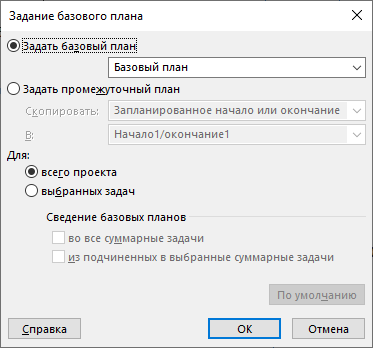
\includegraphics[width=0.7\textwidth]{imgs/task_3_3.png}
	\end{center}
\end{figure}